\newcommand{\InitEtape}[2]{
\node[Etape,label=right:#2] (#1) {};
}
\newcommand{\pEtape}[3]{

\node[Etape,label=right:#2] (#1) {};
\draw[->] (I) -- (T);
}

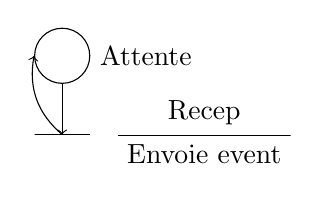
\begin{tikzpicture}\shorthandoff{:}


	\tikzset{Etape/.style={draw,black,minimum size=0.7cm,inner sep=0pt,circle,font=\tiny}}
	\tikzset{Trans/.style={draw,black,minimum width=0.7cm,minimum height=0.0cm,inner sep=0pt,outer sep=0pt,rectangle,font=\tiny}}
	
	\tikzset{Line/.style={path picture={\draw[black] (path picture bounding box.north west) -- (path picture bounding box.north east);}}}


\node[Etape,label=right:Attente] (I) {};
\node[Trans,align=center,below of=I] (T) {};
\node[Line,align=center,anchor=north west,at =(T.east),xshift=10pt, label=above:Recep] {Envoie event};


\draw[->] (I) -- (T);

\draw[->] (T) edge [bend left] (I.west);



\end{tikzpicture}

